\subsection{Hair}

\subsubsection{State of the Art in Hair Rendering}

Hair and fur are ubiquitous in rendered media, from video games to animated film characters. To this day, the realistic rendering of fibers remains challenging, from their geometric complexity to the intricate scattering of light from fiber to fiber. Most modern techniques can be traced back to either the hair card approach proposed by Kajiya and Kay \cite{kajiya1989rendering} or the fiber scattering paradigm that originated with Marschner et al. \cite{marschner2003}. In recent years, research has focused on making the light scattering computation tractable for Monte Carlo path tracers, for example chiang and al. \cite{chiang2016} developed a artist friendly model that is now widly accepted as a practical hair shading model in tools like houdini and Mitsuba3 for example.

\paragraph{Kajiya and Kay Model}

The Kajiya and Kay model (1989)~\cite{kajiya1989rendering} is based on a polygonal hair representation, allowing it to integrate smoothly with commonly used rasterized rendering pipelines. The approach works by modeling hair as cylindrical fibers and using an anisotropic shading model that accounts for the tangent direction of the hair strand.

The model captures the most obvious feature of fiber scattering: the appearance of a linear highlight in the image running perpendicular to the fiber directions. This is based on the observation that reflection from a parallel beam off the surface of a cylinder produces a cone centered on the hair axis. The model combines a diffuse term (proportional to the cosine of the incident angle) with a specular highlight centered on this cone.

However, the Kajiya and Kay model has significant limitations. It treats hairs as opaque cylinders and does not account for transmission or internal reflection. Since hair is a dielectric material, and blonde, brown, red, or other light-colored hair is translucent, this omission leads to a less realistic appearance that fails to capture the colored highlights and backlit transmission seen in real hair.

\paragraph{Marschner Model}

The Marschner model (2003)~\cite{marschner2003} represents a significant advancement over Kajiya and Kay by modeling hair more realistically. The model treats hair fibers as rough dielectric cylinder, enabling proper simulation of internal reflection and transmission.

Marschner established three primary modes of light interaction with hair:

\begin{itemize}[noitemsep]
    \item \textbf{R (Reflection)}: Light reflects off the outer surface of the hair fiber, producing the primary white highlight
    \item \textbf{TT (Transmission-Transmission)}: Light transmits into the fiber, passes through the interior, and exits on the opposite side, creating forward scattering that is visible in backlit conditions
    \item \textbf{TRT (Transmission-Reflection-Transmission)}: Light transmits into the fiber, reflects internally off the back surface, and transmits out again, producing the colored secondary highlight
\end{itemize}

The scattering function can be written as:

\begin{equation}
\begin{aligned}
S(\theta_i, \theta_r, \phi_i, \phi_r) &= \frac{M_R(\theta_h) N_R(\eta'(\eta, \theta_d), \phi)}{\cos^2(\theta_d)} \\
&+ \frac{M_{TT}(\theta_h) N_{TT}(\eta'(\eta, \theta_d), \phi)}{\cos^2(\theta_d)} \\
&+ \frac{M_{TRT}(\theta_h) N_{TRT}(\eta^*(\phi_h, \theta_d), \phi)}{\cos^2(\theta_d)}
\end{aligned}
\end{equation}

where $M$ represents the longitudinal scattering function (modeled as Gaussians) and $N$ represents the azimuthal scattering function. The model uses spherical coordinates with $\theta$ representing the longitudinal angle and $\phi$ representing the azimuthal angle. Several derived angles are employed:
\begin{itemize}
    \item The difference angle: $\theta_d = (\theta_r - \theta_i)/2$
    \item The relative azimuth: $\phi = \phi_r - \phi_i$
    \item The half angles: $\theta_h = (\theta_i + \theta_r)/2$ and $\phi_h = (\phi_i + \phi_r)/2$
\end{itemize}
In principle, this pattern could be extended to all sets of transmissions with $n$ internal reflections (e.g., TRRT, TRRRT, etc.), but the visual impact of higher-order terms beyond TRT is not significant for most applications, as they carry progressively less energy.



% TODO: EXPLAIN M and N scattering functions


\subsubsection{Comparison of Hair Rendering}

The figure \ref{fig:hair_comparison} shows on the left hair shaded using the Kajiya-Kay model, in the middle using the Marschner model and on the right real hair under similar lighting conditions. We can clearly see that the Marschner model enables better representation of the second colorful highlights by giving it a less flat look than the Kajiya model, yet it still presents a uniform look that doesn't exactly capture the appearance of real hair.

\begin{figure}[H]
    \centering
    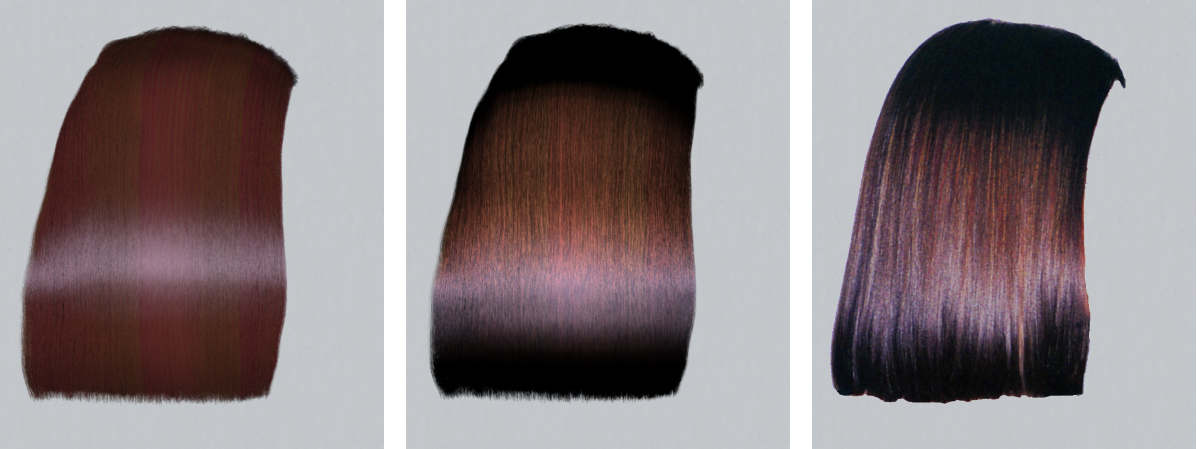
\includegraphics[width=\textwidth]{img/hair_comparison.png}
    \caption{Comparison of hair rendering models: Kajiya-Kay model (left), Marschner model (middle), and real hair (right) under similar lighting conditions. Image from \textcite{marschner2003}.}
    \label{fig:hair_comparison}
\end{figure}
